\chapter{Adaptive time-tree transition kernels for Bayesian phylogenetics}

\section{Introduction}	
\label{sec:intro}

The use of Markov chain Monte Carlo (MCMC) for Bayesian methods in phylogenetics has grown steadily since its introduction in the late 1990s and early 2000s~\citep{Rannala1996, Yang1997, Mau1999, Li2000}, with software packages such as Mr Bayes~\citep{Ronquist2012} and BEAST~\citep{Drummond2012} becoming widely used by researchers in a broad range of disciplines~\citep{Murphy2001, Bouckaert2012, Lemey2014}.
% \citep{sinsheimer1996bayesian} is probably the first use of Bayesian methods in phylogenetics.

In Bayesian phylogenetics one is usually interested in computing the posterior distribution
\begin{equation}
\label{eq:posterior}
 p(t, \boldsymbol b, \boldsymbol \theta | D) = \frac{f(D | t, \boldsymbol b, \boldsymbol \theta ) \pi(t, \boldsymbol b, \boldsymbol \theta )}{\sum_{t_i \in \boldsymbol T} \int_{\boldsymbol B}\int_{\boldsymbol \Theta} f(D | t_i, \boldsymbol b_i, \boldsymbol \theta ) \pi(t_i, \boldsymbol b_i, \boldsymbol \theta ) d\boldsymbol\theta d\boldsymbol b_i}\:,
\end{equation}
where $D$ is observed data, $\boldsymbol T$ is the set of all binary rooted trees and $t \in \boldsymbol T$  is a tree topology associated set of branch lengths $\boldsymbol b$.
Finally $\boldsymbol \theta$ is a set of parameters of interest such as substitution model parameters, migration rates, heritability coefficients, etc.

In many applications, interest lies in constructing time-calibrated phylogenies, i.e. phylogenetic trees whose branch lengths are measured in units of calendar time.
In particular, one might have sequences sampled through time (heterochronous) which enable direct estimation of the rate of evolution and reconstruction of past population dynamics~\citep{Drummond2002, Drummond2005}.
These types of data sets pose additional challenges to inference because they impose constraints on the space of valid trees~\citep{Stadler2013}.

One of the main features of the Bayesian  approach is to  allow parameter inference and hypothesis testing whilst accommodating phylogenetic uncertainty~\citep{Suchard2001, Huelsenbeck2002}.
This treatment of uncertainty is achieved by integrating over the space of phylogenies, which depends crucially on efficiently traversing tree space.
Even for the simplest models, the distribution in~(\ref{eq:posterior}) cannot be computed analytically, requiring numerical approximation, usually  accomplished through MCMC.

The Metropolis-Hastings (M-H) algorithm~\citep{Metropolis1953, Hastings1970} is a very popular MCMC technique due to its generality and ease of implementation.
In M-H, a Markov chain is constructed such that its limiting distribution is the desired posterior distribution. 
For ease of presentation, let $\tau = \{ t, \boldsymbol b\}$ and $q_{\gamma}(\tau^\prime|\tau)$ be a conditional distribution indexed by a parameter $\gamma$ from which a new state $\tau^\prime$ can be proposed from a current state $\tau$, which we call a \textbf{tree transition kernel}. 
It can be shown that accepting/rejecting a new state $\tau^\prime$ based on the ratio $A_{\gamma}(\tau | \tau^\prime) = min\left(1, \frac{p(\tau^\prime | D)q_{\gamma}(\tau|\tau^\prime)}{p(\tau | D)q_{\gamma}(\tau^\prime|\tau)}\right)$ leads to the desired distribution for a suitably constructed tree transition kernel.

An important thing to notice is that there are no ``default'' choices for the proposal distribution $q_{\gamma}(\cdot|\cdot)$; it must be chosen with the target posterior in mind.
Moreover, the efficiency of MCMC algorithms in approximating the target distribution depends crucially on the choice of transition kernel~\citep{Brooks2003,AlAwadhi2004,Yang2013}.
As argued by~\cite{Hoehna2012}, tree transition kernels are usually built in a relatively simplistic fashion, which in turn leads to inefficient exploration of tree space.
Moreover, most transition kernels proposed to date are not adaptive, i.e., the parameter(s) $\gamma$ cannot be adjusted during the Markov chain to achieve a desired acceptance probability.
Given the clear advantage of adaptive MCMC over non-adaptive implementations for high-dimensional target distributions~\citep{Roberts2009, Baele2017}, the development of adaptive tree transition kernels could lead to substantial gains in performance.

\cite{Lakner2008} were the first to systematically investigate transition kernel efficiency in MCMC for Bayesian phylogenetics.
They investigated the performance of seven kernels on a collection of 10 real-world data sets.
To quantify performance, the authors looked at the percentage of converged runs per tested kernel, using clade frequencies relative to a reference (golden) run as a criterion.
In addition, time to convergence was also used as performance criterion.

\cite{Hoehna2008} developed new ``clock-constrained'' transition kernels to improve efficiency when dealing with time-calibrated trees. 
The authors argue that clock-constrained trees impose additional restrictions on the state space of the MCMC algorithm and hence that performance could be increased by developing transition kernels that took the extra information provided by tip dates.
They develop two such kernels: Fixed node-height Prune-and-Regraft (FNPR) and Intermediate Exchange (IE).
FNPR finds a ``target'' node (excluding the root and its two daughters) at random, prunes it and regrafts the resulting subtree at a ``destination'' node in the tree at the same height at random.
Intermediate Exchange is similar in spirit, but the regraft node  is not chosen at random. 
Instead, IE is constructed to prefer local rearrangements, by picking closer nodes with a higher probability (see below and section II in~\cite{Hoehna2008} for details).
A limitation of FNPR nor IE is that they are not adaptive.

\cite{Hoehna2012} explored more sophisticated ``guided'' tree transition kernels, inspired by Gibbs sampling.
The idea behind their ``metropolised'' Gibbs samplers is to maximise transition probability, i.e., the probability that the chain moves to a new state.
This is accomplished by prohibiting the current state as a proposed state, leading to a transition probability of one.
The kernels developed in~\cite{Hoehna2012} use a weighting scheme based on conditional clade probabilities (CCP) to guide transitions between trees.
A move to a tree with a lower CCP score is thus less likely, whilst a move that increases the score has a higher probability of being accepted.
A limitation of these metropolised transition kernels is that CCP scores require normalisation over all trees~\citep{Larget2013} and hence can be cumbersome to calculate.

To achieve maximum efficiency, a tree transition kernel needs to have the following characteristics: (i) be computationally cheap; (ii) be adaptive; (iii) traverse tree space quickly.

In this paper we develop and study a suite of simple, adaptive time-tree transition kernels, which we implement in the open source software package BEAST (\url{https://github.com/beast-dev/beast-mcmc/}).
We analyse performance in real as well as simulated data sets, focusing on the inference of time-calibrated phylogenies.


\section*{New time-tree transition kernels}


\section*{Results}

\begin{figure}[htbp]
  \centering
  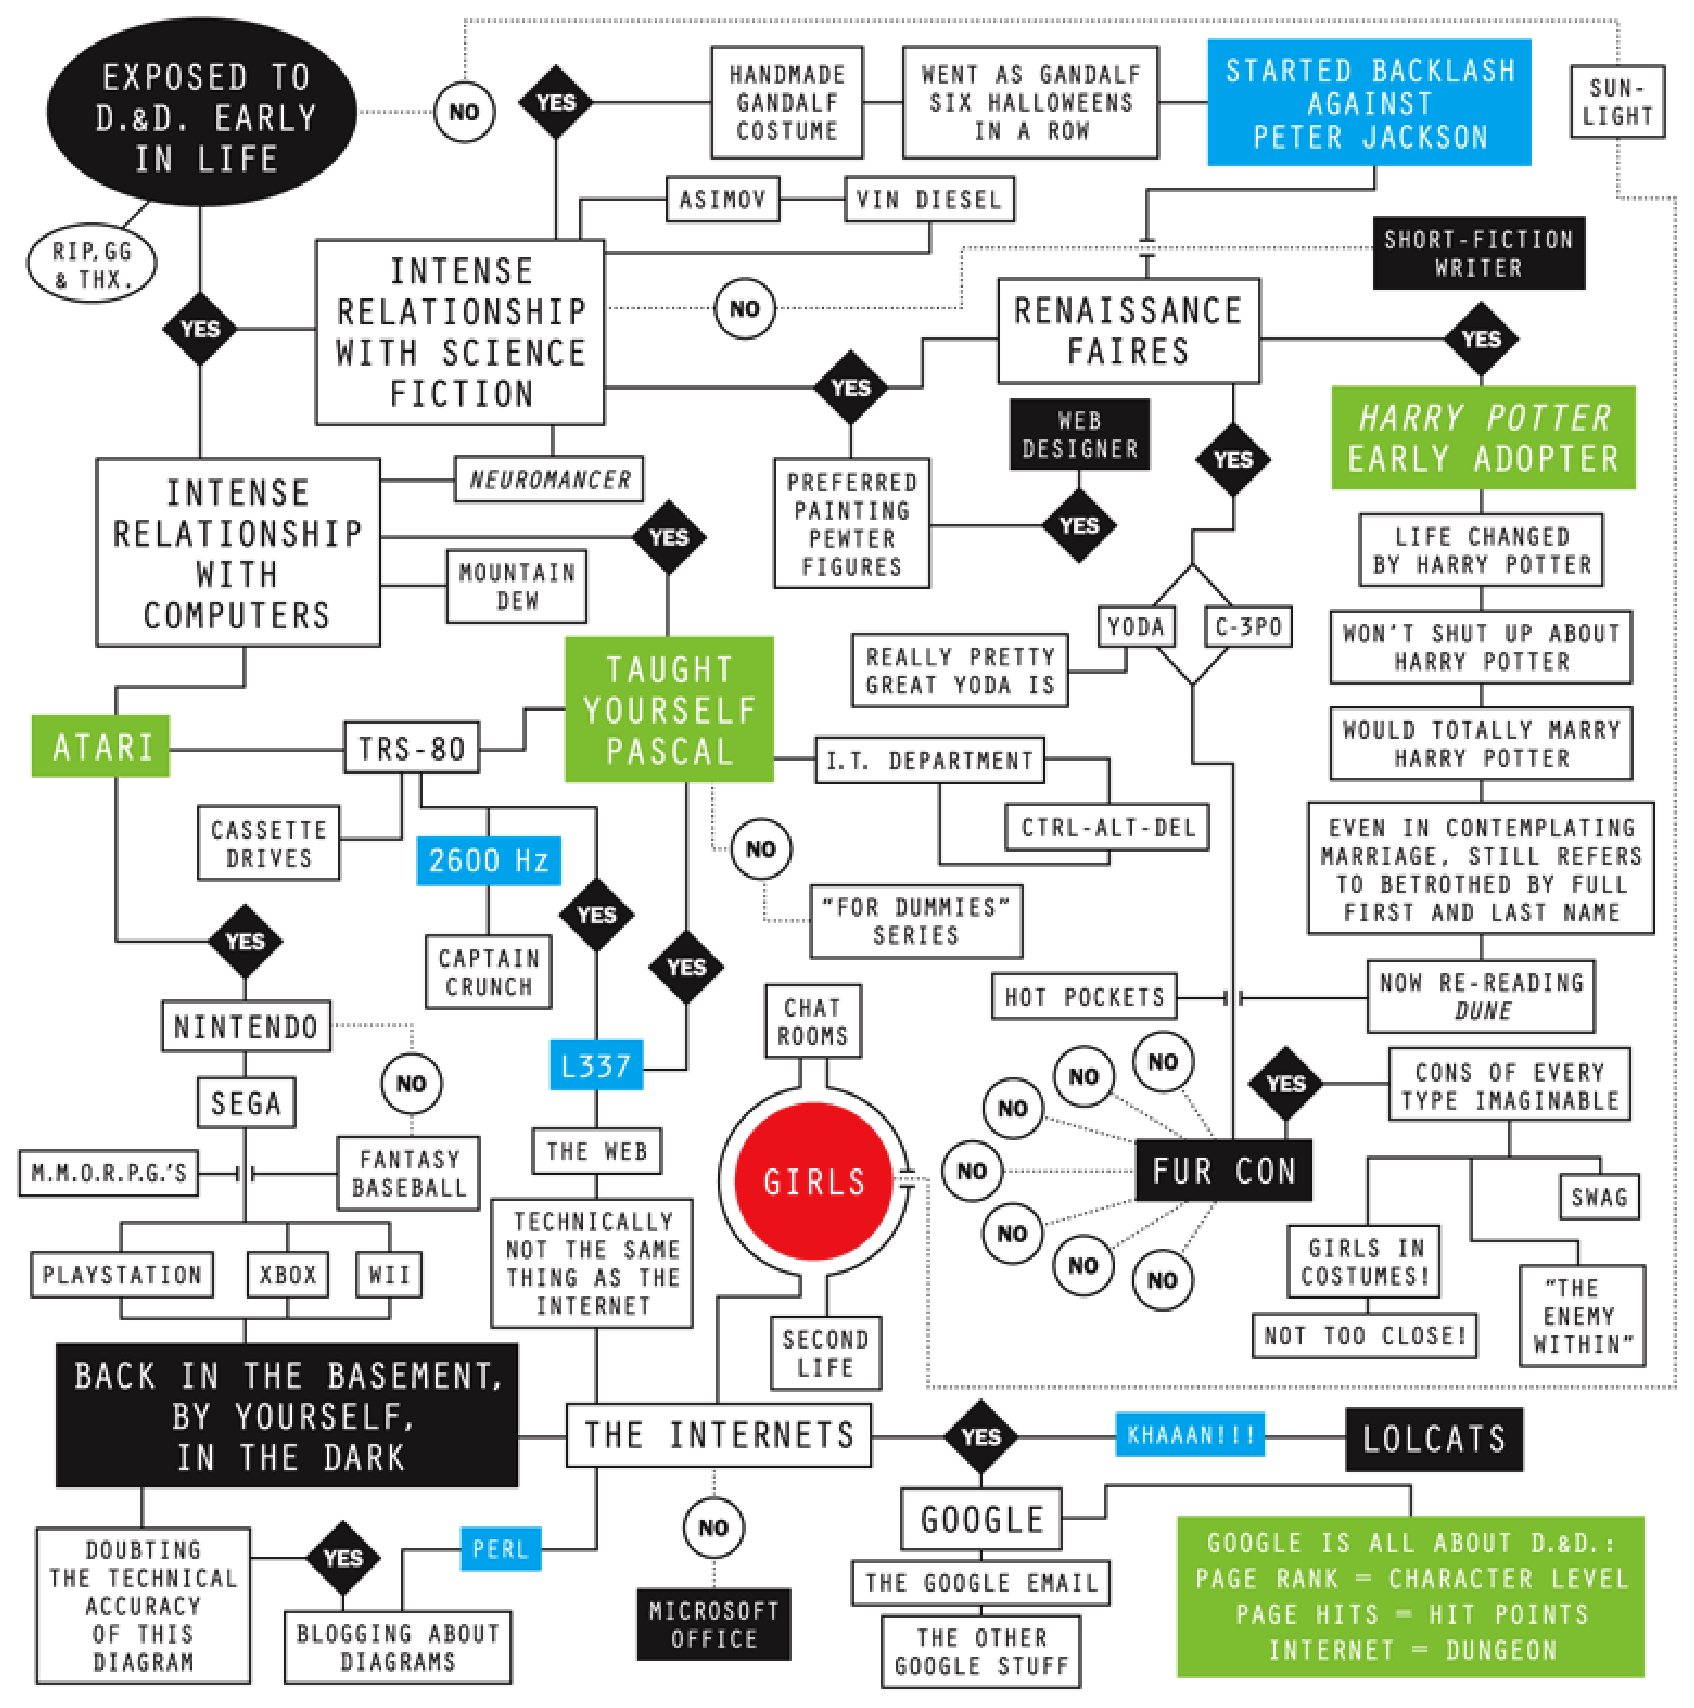
\includegraphics[width=0.7\textwidth]{\dir/figs/geek_flow_chart_nyt.eps}
  \caption{an example figure...}
  \label{fig.example}
\end{figure}

% \bibliography{/home/max/Dropbox/PHD/THESIS/bibliography/lmcarvalho_PhD_Thesis}
